\pdfoutput=1
% In particular, the hyperref package requires pdfLaTeX in order to break URLs across lines.

\documentclass[11pt]{article}

% Change "review" to "final" to generate the final (sometimes called camera-ready) version.
% Change to "preprint" to generate a non-anonymous version with page numbers.
\usepackage[preprint]{acl}

% Standard package includes
\usepackage{times}
\usepackage{latexsym}

% For proper rendering and hyphenation of words containing Latin characters (including in bib files)
\usepackage[T1]{fontenc}
% For Vietnamese characters
% \usepackage[T5]{fontenc}
% See https://www.latex-project.org/help/documentation/encguide.pdf for other character sets

% This assumes your files are encoded as UTF8
\usepackage[utf8]{inputenc}

% This is not strictly necessary, and may be commented out,
% but it will improve the layout of the manuscript,
% and will typically save some space.
\usepackage{microtype}

% This is also not strictly necessary, and may be commented out.
% However, it will improve the aesthetics of text in
% the typewriter font.
\usepackage{inconsolata}

%Including images in your LaTeX document requires adding
%additional package(s)
\usepackage{amsmath}
\usepackage{amsfonts}
\usepackage{geometry}
\usepackage{graphicx}
\usepackage{float}
\usepackage{cleveref}


\usepackage{tabularx}             % For flexible-width columns
\usepackage{booktabs}             % For nicer table rules
\usepackage{array}                % Extended col types if needed

% If the title and author information does not fit in the area allocated, uncomment the following
%
%\setlength\titlebox{<dim>}
%
% and set <dim> to something 5cm or larger.

\title{Instructions for *ACL Proceedings}

\usepackage{hyperref}

\newcommand{\links}{\textbf{\textsc{Links}}}
\newcommand{\recorder}{\textregistered}
\newcommand{\studentmodel}{\studentmodel}
\newcommand{\teachermodel}{\teachermodel}
\newcommand{\mnemonic}{$m$}
\newcommand{\mnemonics}{$m$'s}
\newcommand{\vocabulary}{$v$}
\newcommand{\eg}{$e$}

\author{%
  My (Chiffon) Nguyen \\
  College of Computational Sciences \\
  Minerva University \\
  San Francisco, CA 94108 \\
  chiffonng@uni.minerva.edu
}

\begin{document}

\begin{titlepage}
\centering
{\scshape\LARGE Minerva University \par}
\vspace{1cm}
\begin{center}
    
\includegraphics[width = 0.4\linewidth]{figures/minerva_logo.png}
\end{center}
{\scshape\Large Capstone: Class of 2025 \par}
\vspace{1.5cm}
{\huge\bfseries LINKS: Generate linguistically grounded mnemonic devices for English vocabulary learning with reasoning, multilingual LLMs \par}
\vspace{2cm}
{\scshape\large Tra My Nguyen \par}
submitted in partial fulfillment of the requirements for the degree of Bachelor of Science in Computational Sciences \par
\vspace{2cm}
{\large\itshape Capstone Committee \par}
Dr. Patrick Watson \\
Dr. Philip Sterne

\vfill
{\large \today\par}
\end{titlepage}

\onecolumn
\section*{Executive Summary}
Note: Due to limited compute, some experiments conducted are small-scale and need more data for robust validation and conclusion. However, the codebase is reproducible and scalable when there is more compute.

Tags: computational linguistics, natural language processing, large language model, language education, english as a foreign language, vocabulary acquisition, synthetic data generation.

\clearpage

\tableofcontents
\clearpage

\twocolumn

\maketitle
\begin{abstract}
To acquire advanced vocabulary, English learners often use mnemonic devices, memorable associations linking a new concept to learned concepts to improve memory and recall. Reviewing the literature on mnemonic techniques, we characterize good mnemonics as \textbf{linguistically grounded}, which better link to the target vocabulary, improving long-term retention and linguistic knowledge, especially at advanced levels (CEFR B2+). We investigate whether Large Language Models can consistently help write such effective mnemonics, with three different settings: in-context learning, and reasoning distillation. Concretely, we first measured different prompting strategies with a frontier reasoning model, \teachermodel, and generated \links, a synthetic dataset of 2000 triplets of \textit{reasoning trace, mnemonic, and example sentence} for 2000 vocabulary useful for TOEFL iBT \footnote{Internet-based Test of English as a Foreign Language}, IELTS Academic \footnote{International English Language Testing System}, and SAT\footnote{Scholastic Aptitude Test}. Second, using a subset of \links, we distilled linguistic reasoning from the \textit{teacher model} to the \textit{student model}, \studentmodel\footnote{https://huggingface.co/collections/google/gemma-3-release-67c6c6f89c4f76621268bb6d} , with online reinforcement learning. The trained, quantized model can be served with a local application such as OpenWebUI (interface) and Ollama (command-line).

Preliminary evaluation shows

The project examplifies that carefully designed NLP systems can generate resources for language learning, either in classroom settings or in self-study. Code, models, and dataset are available\footnote{Links: \href{https://github.com/chiffonng/mnemonic-gen}{Github codebase} and \href{https://huggingface.co/collections/chiffonng/vocab-mnemonic-mining-67563a0a1ab91e84e9827579}{HuggingFace collection of datasets and artifacts}}.
\end{abstract}

\section{Introduction}
Vocabulary acquisition challenges many English language learners, particularly at upper intermediate to advanced levels where abstract and academic vocabulary predominates. Mnemonics, cognitive tools that help learners create associations between new vocabulary and familiar concepts, serve as valuable tools for enhancing retention and recall. The deeper learners elaborate the connection between the mnemonic and the target vocabulary, the longer and better they can recall the term. However, creating such effective mnemonics demands both linguistic expertise and creative effort, presenting a significant barrier for most learners. Large Language Models (LLMs) have demonstrated capabilities as knowledge bases and creative text generators, suggesting their potential for automated mnemonic generation.

Previous work explored automated mnemonic generation through computational methods using the \textbf{keyword method}, which involves 1) generateing simpler keywords that together sound or look like the target vocabulary and 2) creating memorable explanations that include the vocabulary, the keywords, amd its meaning \citep{atkinsonApplicationMnemonicKeyword1975}. \citet{savvaTransPhonerAutomatedMnemonic2014} and \citet{OzbalAUTOMATION2014} generated keywords of phonetic and orthographic similarities in the native language for foreign language vocabulary, across multiple languages. \citet{LeeSMARTPHONE2023} extended this work and utilized LLMs to produce phonetically similar keywords and visual cues and \citet{LeeEXPLORING2024} prompted LLMs to generate multiple mnemonic candidates and evaluate them based on imageability and coherence. Most recently, \citet{balepurSMART2024} fine-tuned LLaMA-2-70B on 800 crowd-sourced mnemonics and aligned outputs with learner preferences and learning outcomes.

%%%% Figure Highlight the difference between keyword "mnemonic" and "linguistically grounded mnemonics" with an example
%%% (e.g., \textbf{preposterous} can be broken down as pre- (before) + poster (after) + ous. Anything that comes both before and after is preposterous)

Although the keyword method is commonly used and empirically validated in classroom and laboratory contexts \citetext{\citealp{atkinsonApplicationMnemonicKeyword1975}, \citealp{pressleyMnemonicKeywordMethod1982}}, it may lead to longer retrieval time \citep{vanhellKeywordMnemonicsRote1997} and be inadequate for fairly abstract vocabulary \citetext{\citealp{camposLimitationsMnemonicKeywordMethod2003}, \citealp{camposImportanceKeywordGenerationMethod2004a}}. Such methods typically neglect other rich linguistic knowledge embedded in LLMs that could provide diverse mnemonic strategies beyond simple keyword associations. Second, previous works passively deliver generated mnemonics to learners. While \textsc{Smart} \citep{balepurSMART2024} was further trained on learners' preferences, these preferences were aggregated, potentially missing alignment with individual learning styles. Language learners who use self-created mnemonics retain vocabulary more effectively and for longer duration \citep{madanExploringWordMemorability2021}.

Our contributions can be summarized as follows. (\textbf{1}) We demonstrate that LLMs can generate \textbf{linguistically grounded mnemonics}, which emphasizes the importance of linguistic features in creating effective mnemonics, through reasoning and creative writing. (\textbf{2}) We present \links, a synthetic dataset of 2000 triplets of \textit{reasoning trace, mnemonic, and example sentence} for 2000 vocabulary. They can be integrated in a spaced repetition system (SRS) or language learning applications for vocabulary acquisition with better retrieval. (\textbf{3}) We distill the reasoning capabilities of a frontier, reasoning LLM, into a smaller model, \studentmodel, using \citep{DeepSeek-AIDEEPSEEKR12025}. The trained model \links, can be served locally, enabling users to generate mnemonics without relying on external APIs or internet connectivity.

\section{Background}

We assume a background on LLMs, including their transformer-based architecture (\Cref{app:llm-transformer}), in-context learning (\Cref{sec:icl-performance}), and reinforcement learning (full preliminaries are provided in \Cref{app:technicality}). We briefly review the literature on mnemonic devices for vocabulary learning and the use of LLMs in linguistic tasks.

\subsection{Mnemonic devices for vocabulary learning}

\begin{table*}[htb]
\centering
\caption{Examples of feature categories for English words.}
\label{tab:linguistic-features}
\begin{tabularx}{\textwidth}{l >{\raggedright\arraybackslash}X >{\raggedright\arraybackslash}X}
\toprule
\textbf{feature} & \textbf{description} & \textbf{example} \\
\midrule
\textbf{phonetics} & vocab's sound patterns & \emph{apparent} sounds like “a bare Asian.” \\
\addlinespace
\textbf{orthography} & written/spelling patterns & \emph{abet} looks like “a + bet.” \\
\addlinespace
\textbf{morphology} & structure including free and bound morphemes & \emph{aggrandize} = a + grand + –ize, to mean to make grander. \\
\addlinespace
\textbf{etymology} & vocab origin and history & \emph{adumbrate} comes from Latin ad- (to, on) + umbra (shade) + ate, to mean foreshadow or outline. \\
\addlinespace
\textbf{semantics} & vocab meaning and relationships & \emph{confound} has similar meaning and history with 'confuse'. \\
\bottomrule
\end{tabularx}
\end{table*}

\subsection{LLMs: linguistic competence and creativity}

\section{In-context learning performance} \label{sec:icl-performance}

%% TODO: Review in-context learning literature here, including CoT, few-shot prompting, and zero-shot prompting. Discuss the differences between these methods and their implications for LLMs' performance in generating mnemonics.
\subsection{Experimental setup}
We systematically compared various in-context learning approaches to understand how different prompting techniques affect mnemonic generation. \Cref{fig:prompting-methods} illustrates the percentage of linguistically grounded mnemonics generated by different prompt formulations.

We used \verb|curator| \citep{BespokeLabBESPOKE2025} with \verb|litellm| orchestration layer to interact with LLM APIs, simpify API calls, manage rate limits, and handle retries.

\subsection{Results}

\begin{figure}
  \centering
  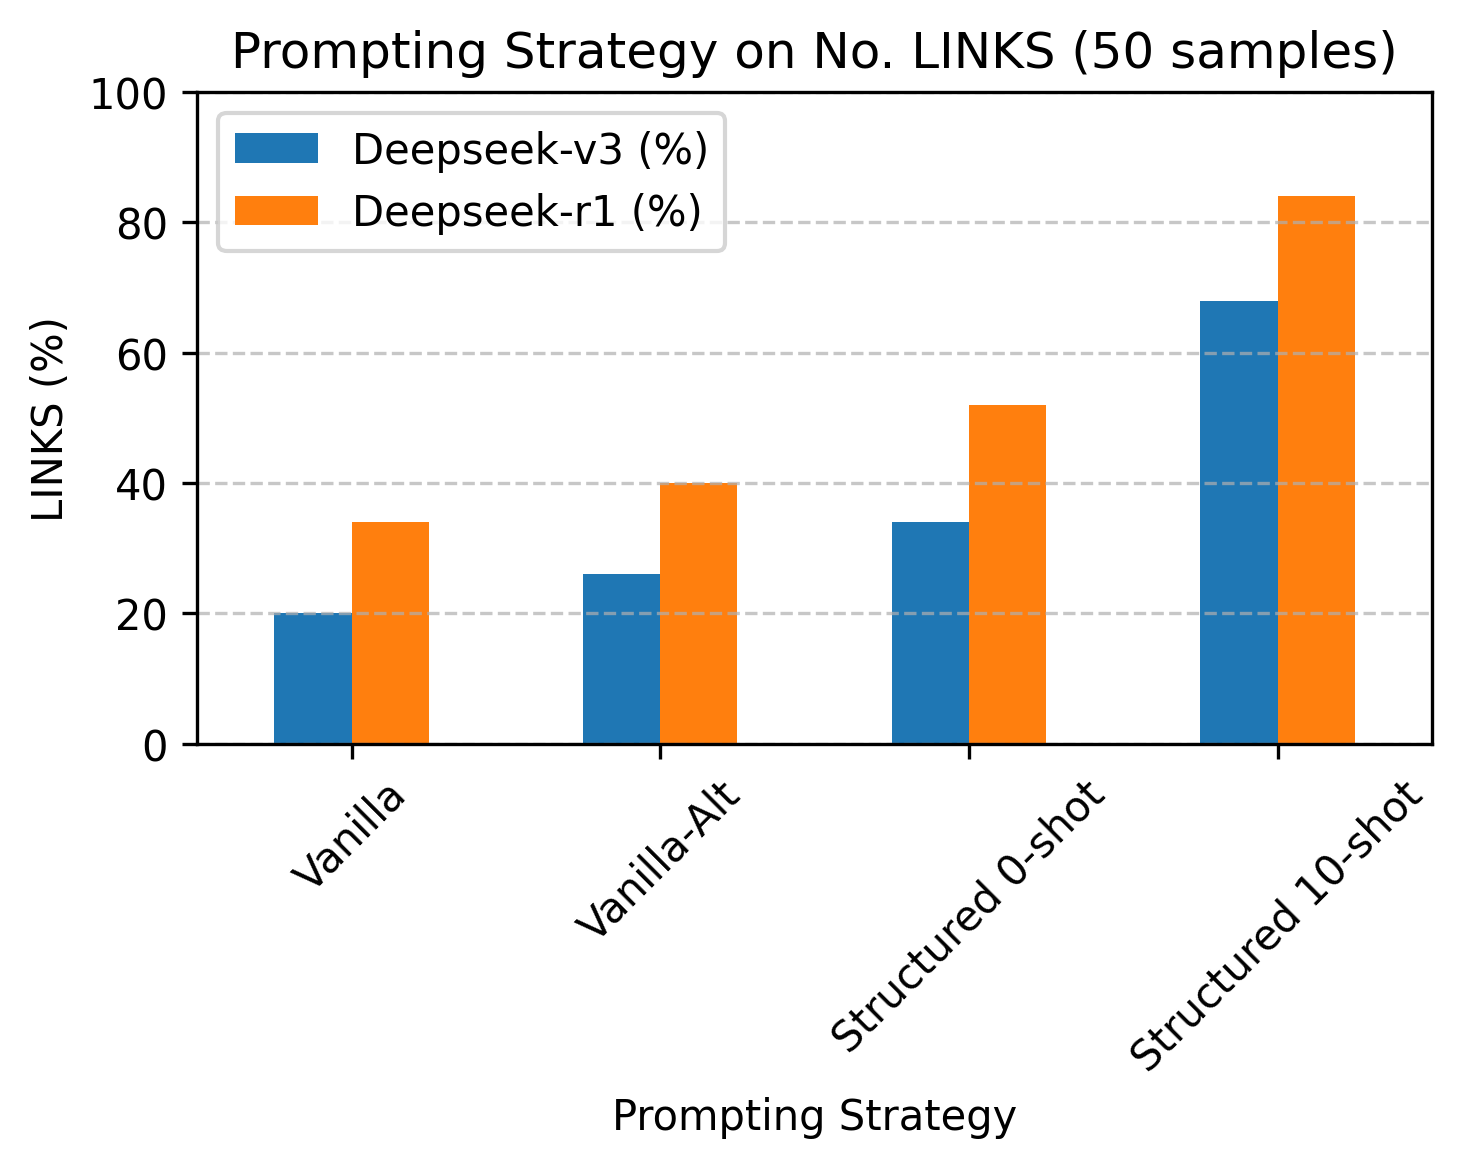
\includegraphics[width=\linewidth]{figures/prompt_comparison.png}
  \caption{Comparison of prompting methods (see detailed prompt in \Cref{app:prompt-usage}). Y-axis shows percentages of linguistically-grounded mnemonics generated out of 50 requests sent for each prompt type.}
  \label{fig:prompting-methods}
\end{figure}

We observed significant variation in the quality and linguistic grounding of generated mnemonics based solely on prompt formulation. Four distinct prompting strategies were evaluated (see details in \cref{app:prompt-usage})
Vanilla
Reasoning LLMs tend to overthink \citep{xuChainDraftThinking2025}
Good practices: provide decomposed instructions, structured output format, demonstration examples \citep{MishraREFRAMING2022}, and clarify definitions of linguistic features \citep{yinDidYouRead2023}

compress task definition \citep{yinDidYouRead2023},


\section{Knowledge and reasoning distillation} \label{sec:distillation}

%% \begin{figure}
%%   \centering
%%   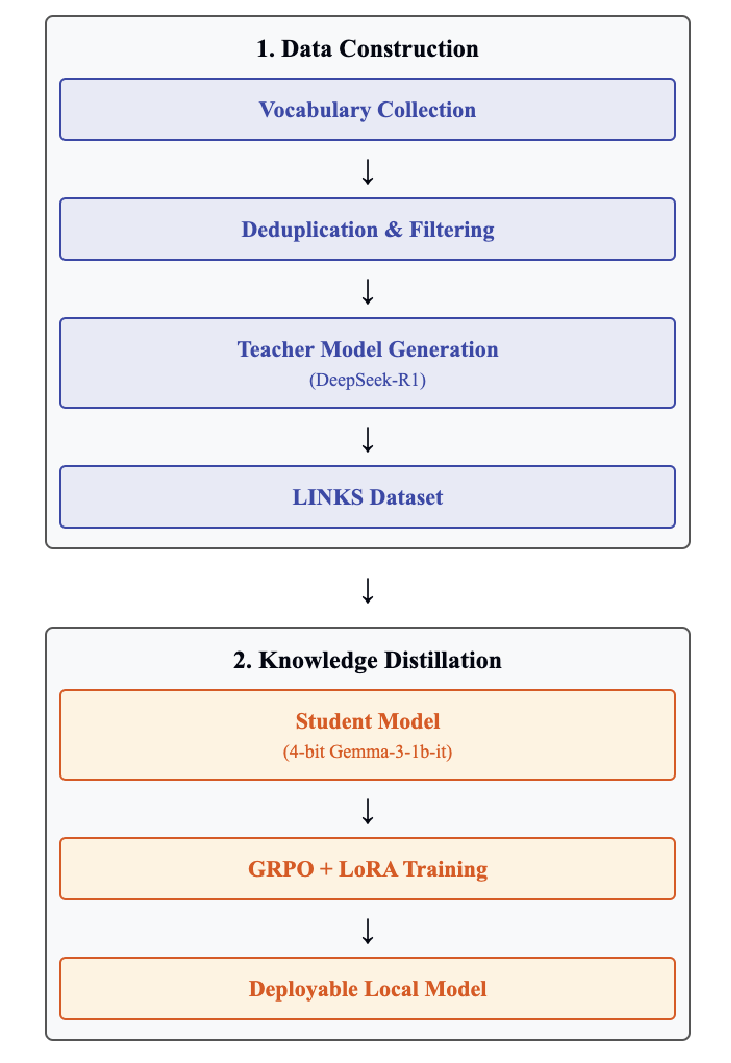
\includegraphics[width=\linewidth]{figures/pipeline.pdf}
%%   \caption{\links pipeline. The pipeline consists of two main components: (1) CoT data generation and (2) model distillation. In the first step, we generate a dataset of mnemonics with reasoning traces using a large language model (LLM) as a teacher. In the second step, we distill the reasoning capabilities of the teacher model into a smaller student model using GRPO \Cref{app:grpo}. The final model can be deployed locally for vocabulary learning tasks.}
%%   \label{fig:distillation}
%% \end{figure}

We present \links, a pipeline that distills linguistic knowledge and reasoning through a teacher-student framework. This approach generates linguistically grounded mnemonics with reasoning traces and exemplifying sentences for vocabulary learning.

\subsection{Data construction} \label{sec:data-gen}
To generate high-quality linguistically grounded mnemonics, we first created a comprehensive training dataset. Following best practices in synthetic data generation with LLMs \citetext{\citealp{longLLMsDrivenSyntheticData2024b}, \citealp{openthoughtsteamOpenThoughts2025}}, we designed a data construction pipeline with several key components.

\paragraph{Vocabulary collection} We collected 5,000 distinct vocabulary words from four complementary sources: English as a foreign language tests (TOEFL iBT, IELTS Academic), standardized tests (SAT, GRE), CEFR levels C1 and C2 word lists, and the Oxford Dictionary of Philosophy. We selected these sources to ensure coverage of academic and abstract vocabulary that would benefit from mnemonic devices. After deduplication and fuzzy-matching decontamination, we refined our dataset to 2,000 distinct vocabulary words for post-training.

\paragraph{Prompt design} Based on the findings from \cref{sec:icl-performance}, we crafted system and user prompts that encouraged linguistically grounded reasoning. Our system prompt instructed the model to analyze potential linguistic features before generating a mnemonic. We used structured output format with designated sections for reasoning, mnemonic, and example, allowing for clearer evaluation and potential future extraction of specific components.

\paragraph{Teacher model selection} We selected \teachermodel (670B parameters) \citep{DeepSeek-AIDEEPSEEKR12025} for its advanced reasoning capabilities and extensive knowledge as the teacher model.

\paragraph{Dataset generation} Using the designed prompts and vocabulary list, we generated the \links, a dataset of approximately 2,000 entries, each containing: (1) a detailed reasoning trace exploring multiple linguistic features of the target vocabulary, (2) a concise mnemonic device leveraging the most salient linguistic connection, and, (3) an exemplifying sentence demonstrating proper usage.

\paragraph{Quality control} To ensure the quality of the generated mnemonics, we implemented a multi-step validation process. We first filtered out any entries that did not meet our structured output format or contained incomplete reasoning traces. We then performed a manual review of a random sample of 200 entries to assess the linguistic grounding and coherence of the mnemonics. This review process involved checking for clear connections between the vocabulary and the mnemonic, as well as ensuring that the example sentence accurately reflected the vocabulary's meaning.

\subsection{Training and inference}
After generating the synthetic dataset, we implemented a distillation process to transfer this linguistic reasoning capability to a smaller, easier-to-deploy model.

\paragraph{Student model selection} We selected \studentmodel as our student model due to its balance of performance, size, and deployment flexibility. This instruction-tuned variant of Google's Gemma-3 (1 billion parameters) \citep{GemmaTeamGEMMA2025} offers several advantages: (1) demonstrated instruction-following abilities, (2) multilingual capabilities for potential cross-lingual applications, and (3) compact size enabling deployment on consumer hardware including Apple Silicon.

\paragraph{Group Relative Policy Optimization (GRPO)} We employed GRPO \citep{DeepSeek-AIDEEPSEEKR12025} to distill the reasoning capabilities of the teacher model into the student model. The GRPO process consists of three main steps: (1) generating multiple candidate outputs for each input, (2) scoring these outputs using a reward model(s), and (3) updating the student model's policy based on the scores. GRPO technical details are included in \Cref{app:grpo}  and our used configuration is provided in \Cref{app:grpo}.

We defined three reward functions that encode basic characteristics of effective mnemonics:
(1) adherence to the structured format with reasoning, mnemonic, and example,
(2) explicit incorporation of linguistic features in \Cref{tab:linguistic-features}, and
(3) usage of the target vocabulary in the mnemonic,  penalizing bad mnemonics such as acronyms.
These reward functions operate directly on model outputs, assigning scalar scores based on how well the generation satisfies each criterion. The scores are then combined using weighted summation, with higher weights assigned to criteria 1 and 2.

\paragraph{Training implementation} We trained  using rank-stabilized LoRA \citep{kalajdzievskiRankStabilizationScaling2023}, a parameter-efficient fine-tuning method that maintains stability for adapters with higher ranks. The training configuration used LoRA rank 8, a learning rate of 3e-5, and a cosine learning rate schedule with 10\% warmup ratio. We generated two candidate outputs per training example to enable reinforcement from comparisons. Training was performed on a single NVIDIA A100 GPU over approximately 6 hours.

\paragraph{Model quantization and serving} To enable efficient deployment on consumer hardware, we quantized the final model using 4-bit quantization with the NormalFloat (NF4) data type \citep{dettmersQLoRAEfficientFinetuning2023}. This significantly reduced the model size while maintaining performance quality. The quantized model can be served with a local application such as OpenWebUI (interface) and Ollama (command-line), making it accessible for language learners without requiring continuous internet connectivity or sharing potentially sensitive language learning data with third-party services.

\section{Evaluation}
\subsection{Experimental setup}

\paragraph{LLM-as-a-judge for 1-5 Likert ratings}

\paragraph{Pairwise preference using double-blind annotation}

\paragraph{Interactive side-by-side comparison}

\subsection{Results}

\section{Related work}
\section{Discussion}
\section{Conclusion}
\section{Limitations}

\section*{Acknowledgements}
% Bibliography entries for the entire Anthology, followed by custom entries
\bibliography{custom}
% Custom bibliography entries only
%\bibliography{anthology,custom}

\clearpage
\appendix
\crefname{section}{Appendix}{Appendices}
\Crefname{section}{Appendix}{Appendices}


\section{Prompt usage} \label{app:prompt-usage}

All of the prompts include

\paragraph{Vanilla vs. Alternative Phrasing} When comparing "Generate a mnemonic to help learn and remember the meaning of English vocabulary and how it is written: \{term\}" against "Generate a memory cue to help learn and remember the meaning of English vocabulary and how it is written: \{term\}", we observed substantial differences in output quality. This highlights the word importance effect noted by \citet{hackmannWordImportanceExplains2024}, where specific terms like "mnemonic" may have acquired pre-training biases that associate them primarily with acronyms or keyword methods rather than broader linguistic strategies.

\paragraph{Structured Prompting} We found improved performance with structured prompts that explicitly request linguistic analysis: "Generate a linguistically grounded mnemonic to help me learn and remember the meaning of English vocabulary and how it is written: \{term\}. Think in short traces and stop when you have a good linguistic connection. You must use that linguistic feature to form a mnemonic for the word." This approach yielded a higher percentage of mnemonics with clear linguistic association.

\paragraph{Chain-of-Thought (CoT) Prompting} Incorporating chain-of-thought reasoning by providing both the instruction and examples of step-by-step linguistic analysis significantly improved the quality of generated mnemonics. Our implementation used 10 human-written examples, each demonstrating the process of finding linguistic association of the vocabulary before constructing a mnemonic.

\paragraph{Concise Reasoning Traces} Inspired by \citet{xuChainDraftThinking2025}, we experimented with prompting models to generate minimal reasoning steps. For example: "Generate a mnemonic for \{term\}. Think step by step, but keep a minimum draft for each thinking step." This approach balanced comprehensive linguistic analysis with efficiency, preventing models from overthinking and/or elaborating on irrelevant aspects.

\section{Annotation details} \label{app:annotation}

\subsection{Double-blind annotation}

\section{Technical preliminaries} \label{app:technicality}

\subsection{In-context learning}

\paragraph{Chain-of-Thought (CoT) prompting} \citep{weiChainofThoughtPromptingElicits2023} is a prompting technique that encourages LLMs to generate intermediate reasoning steps before arriving at a final answer. This approach has been shown to improve performance on complex tasks by guiding the model through a structured thought process.

\subsection{Neural Language Models and Transformer Architecture} \label{app:llm-transformer}

Neural language models are probabilistic frameworks that assign probabilities to sequences of words or subword units, known as tokens. A token is the smallest unit of text that the model processes, which can be as granular as individual characters, subwords, or entire words, depending on the tokenization strategy employed.

Given a sequence of tokens \( \mathbf{x} = (x_1, x_2, \ldots, x_T) \), a language model estimates the joint probability \( P(\mathbf{x}) \) by factorizing it into conditional probabilities:

\[
P(\mathbf{x}) = \prod_{t=1}^T P(x_t \mid x_1, x_2, \ldots, x_{t-1})
\]

At each time step \( t \), the model predicts the next token \( x_t \) based on the preceding sequence \( (x_1, x_2, \ldots, x_{t-1}) \). This autoregressive approach enables the generation of coherent text by sequentially predicting subsequent tokens.

The Transformer architecture underpins many state-of-the-art language models due to its efficiency and capability to model long-range dependencies. It utilizes self-attention mechanisms to weigh the relevance of each token in a sequence relative to others, regardless of their positions. The architecture comprises stacked layers, each including multi-head self-attention and position-wise feed-forward networks, facilitating parallelization and effective learning of complex patterns in data.

\subsubsection{Tokenizer} \label{app:tokenizer}

A tokenizer is a preprocessing tool that converts raw text into tokens, aligning the text with the LM's vocabulary. Tokenizers can employ various strategies, such as word-based, character-based, or subword-based tokenization, each with distinct advantages and use cases.

Byte Pair Encoding (BPE) is a subword tokenization algorithm that operates on the byte representation of text, enabling consistent handling of various scripts and special characters. It iteratively merges the most frequent pairs of adjacent bytes to form subword units, constructing a vocabulary that efficiently represents the training corpus. This method allows the tokenizer to decompose rare words into meaningful subword components, enhancing the model's capacity to process diverse and unseen terms.

For instance, the word "preposterous" might be tokenized into subwords like "pre", "poster", and "ous," facilitating the model's understanding and generation of these subwords in novel contexts. This subword granularity enables the model to generalize across morphologically complex words and out-of-vocabulary words, enhancing its robustness and vocabulary coverage. However, not all subwords are valid morphemes, which can limit the model's ability to capture morphological structure accurately. For instance, \texttt{tiktoken} (OpenAI's tokenizer)\footnote{\href{https://platform.openai.com/tokenizer}{https://platform.openai.com/tokenizer}} recognizes "ephemeral" as a single subword rather than three morphemes ("ept", "hemera", "-al"), because the affixes are not explicitly segmented, and 'epheremal' is a rare word so BPE better learns it as a single token.

\subsection{Family of Fine-Tuning Methods} \label{app:finetuning}
Fine-tuning is the process of adapting a pre-trained model to a specific task T or domain D by updating its parameters on a target dataset \(\mathcal{D}\). This process is crucial for leveraging pre-trained models' knowledge and enhancing their performance on downstream tasks.

There are several approaches to fine-tuning, which can be categorized by: 1. the availability of labeled data (supervised vs unsupervised fine-tuning), 2. the extent of parameter updates (full-parameter vs parameter-efficient fine-tuning), and 3. task. We focus on supervised fine-tuning, which involves minimizing a task-specific loss function over a labeled dataset.

\subsubsection{Supervised Fine-Tuning (SFT)}\label{app:sft}

SFT involves adapting a pre-trained model to a target task by minimizing a task-specific loss function over a labeled dataset. For a dataset \( \mathcal{D} = \{(\mathbf{x}^{(i)}, \mathbf{y}^{(i)})\}_{i=1}^N \), where \( \mathbf{x}^{(i)} \) is the input and \( \mathbf{y}^{(i)} \) is the target output, the objective is to minimize:

\[
\mathcal{L} = \frac{1}{N} \sum_{i=1}^N \ell(f(\mathbf{x}^{(i)}; \theta), \mathbf{y}^{(i)})
\]

where \( f(\mathbf{x}; \theta) \) represents the model's output with parameters \( \theta \), and \( \ell \) is the loss function, typically cross-entropy loss.

\textbf{Instruction-tuning} is a specialized form of SFT where models are trained on datasets comprising instruction-response pairs. This approach enables models to generalize across various tasks described by natural language instructions, enhancing their ability to follow diverse prompts. Formally, an instruction-tuning dataset consists of pairs \( \{(\mathbf{I}^{(i)}, \mathbf{y}^{(i)})\}_{i=1}^N \) or triplets \( \{(\mathbf{I}^{(i)}, \mathbf{x}^{(i)}, \mathbf{y}^{(i)})\}_{i=1}^N \), where \( \mathbf{I}^{(i)} \) denotes the instruction, \( \mathbf{x}^{(i)} \) is the optional input, and \( \mathbf{y}^{(i)} \) is the desired output. The training objective is to minimize the loss:

\[
\mathcal{L} = \frac{1}{N} \sum_{i=1}^N \ell(f(\mathbf{I}^{(i)}, \mathbf{x}^{(i)}; \theta), \mathbf{y}^{(i)})
\]

where \( f \) represents the model parameterized by \( \theta \), and \( \ell \) is the loss function measuring the discrepancy between the model's prediction and the target output.

\subsubsection{Parameter-Efficient Fine-Tuning} \label{app:peft}
Full-parameter fine-tuning updates \textit{all} parameters of a pre-trained model on the target dataset, which can be computationally expensive and memory-intensive for large models. Parameter-efficient fine-tuning (PEFT) methods adjust only a subset of the parameters, reducing computational and storage requirements while maintaining performance.

The most common PEFT method is Low-Rank Adaptation (LoRA), and its variants. They are used in the training process.

\paragraph{Low-Rank Adaptation (LoRA)} decomposes the weight updates into low-rank matrices, reducing the number of trainable parameters. Specifically, for a weight matrix \( W \in \mathbb{R}^{d \times k} \), LoRA introduces two low-rank matrices \( A \in \mathbb{R}^{d \times r} \) and \( B \in \mathbb{R}^{r \times k} \), where \( 0 < r \ll \min(d, k) \). The adapted weight is:

\[
W' = W + \alpha \cdot A B
\]

Here, \( \alpha \) is a scaling factor that controls the contribution of the low-rank adaptation. The rank \( r \) determines the capacity of the adaptation, balancing between expressiveness and efficiency.

LoRA introduces \( 2dr \) trainable parameters (size of \( A \) and \( B \)), which is significantly smaller than the original \( dk \) parameters. This reduction in parameters enables efficient fine-tuning of large models on limited hardware. In practice, LoRA is applied to specific modules of the model, such as attention and feed-forward layers, to balance performance and efficiency.

\paragraph{Rank-Stabilized LoRA (rsLoRA)} modifies the scaling factor in LoRA to improve performance across different ranks. The standard scaling factor \( \gamma_r = \alpha / r \) can slow learning for higher ranks. rsLoRA proposes adjusting the scaling factor to \( \gamma_r = \alpha / \sqrt{r} \), enhancing fine-tuning performance without increasing inference costs.

\subsection{Reinforcement Learning (RL)} \label{app:rl}

\subsubsection{Group Relative Policy Optimization (GRPO)} \label{app:grpo}

Intuively, GRPO generates multiple responses for a given prompt, scores them using reward models, calculates the average reward of the group, and then compares each response's score to the average to determine which are better or worse. The model then updates its policy to favor high-reward responses.

Formally,


\section{Training details} \label{app:training-details}
\subsection{Environment setup}
The training was conducted, alternately, on a NVIDIA Tesla T4 GPU provided for free by Google Cloud (through Google Colab, Kaggle Notebook, or Google Cloud's Deep Learning Virtual Machine image) and a 2xH100 NVIDIA GPU server with RunPod (paid by the author, for detailed costs, see \Cref{app:cost}). The T4 GPU has 16GB of memory, while the H100 GPU has 80GB of memory. The T4 GPU was used for initial experiments and supervised fine-tuning, while the H100 GPU was employed for  more extensive training runs and reinforcement learning. The T4 GPU was used for initial experiments and supervised fine-tuning, while the H100 GPU was employed for more extensive training runs and reinforcement learning.

The training environment was set up using these libraries developed by HuggingFace: \verb|bitsandbytes| library for quantization, \verb|peft| for parameter-efficient fine-tuning, \verb|transformers| for model management. The training process was executed using the \verb|trl| library, which provides tools for pre-training and post-training with transformers (including online RL). \verb|unsloth| was used to reduce memory usage on single-GPU environment. \verb|accelerate| and \verb|deepspeed| were used to manage distributed training across multiple GPUs, while \verb|vllm| was used for fast inference and serving of the trained model, especially during online RL.

The base student model used is Google's \studentmodel, an open-weight 1-billion parameter Transformer-based decoder-only text-to-text model pre-trained to work well on general-purpose tasks in multiple languages, and fine-tuned to increase instruction following capabilities. To save memory, a 4-bit quantized version of the model was used, which reduces the model size and speeds up inference without significantly sacrificing performance.

\subsection{LoRA configuration} \label{app:lora-config}

To reduce computational overhead, we employed Rank-Stabilized LoRA (rsLoRA) scaling. The LoRA configuration parameters were set as follows: rank \( r = 8 \), scaling factor \( \alpha_{\text{LoRA}} = 16 \), and dropout rate of 0. These configurations were applied to both the attention and feed-forward layers.

The rank \( r \) determines the dimensionality of the low-rank adaptation matrices, controlling the number of trainable parameters introduced during fine-tuning. A higher rank allows the model to capture more complex adaptations but increases computational complexity. The scaling factor \( \alpha_{\text{LoRA}} \) modulates the impact of the low-rank updates on the original weights, effectively controlling the contribution of the adaptation matrices to the final model parameters. Setting the dropout rate to zero indicates that no dropout regularization was applied during the LoRA updates, allowing all connections to be utilized during training.


\subsection{GRPO configuration} \label{app:grpo-config}

\section{Costs} \label{app:cost}

\section{Documentation of previous iterations} \label{app:previous-iterations}
\subsection{Fine-tune OpenAI} \label{app:openai-finetune}

\subsection{Fine-tune Gemma-3-4b-it} \label{app:gemma-finetune}

For supervised fine-tuning (SFT), we utilized the \texttt{trl} library with the following hyperparameters: batch size \( b = 16 \), number of epochs \( \text{eps} = 4 \), learning rate \( \alpha = 2 \times 10^{-5} \), weight decay \( \lambda = 0.05 \), and a cosine annealing learning rate scheduler with restarts.

The batch size \( b \) defines the number of training examples processed simultaneously during each forward and backward pass. A batch size of 16 balances computational efficiency and gradient estimation accuracy. Training for 4 epochs (\( \text{eps} = 4 \)) means the model will see the training data a total of four times, which ensures sufficient exposure to the training data without risking overfitting. The learning rate \( \alpha \) controls the step size for weight updates; a value of \( 2 \times 10^{-5} \) is typical for fine-tuning large language models, facilitating gradual convergence. Weight decay \( \lambda \) serves as a regularization term, penalizing large weights to prevent overfitting. The cosine annealing scheduler adjusts the learning rate following a cosine decay pattern, periodically restarting to allow the model to escape local minima and potentially achieve better generalization, compared to linear decay.
\end{document}
